\subsection{POC 2: Auto-Complete Form Inputs for Conference Registration in Indico}

The second prototype aims at connecting Solid with the conference registration module in Indico. When registering for a conference, an \gls{html} form is presented with fields previously defined by the conference manager, who deemed those fields necessary. A form always contains personal information of the name and email address, but is not limited to it and can even range to more sensitive information such as copies of personal identification documents. Information of this type has perfect motivation to remain in the owner's hand and not be stored in a remote data store, uncontrollable and unknown to the registrants.

Therefore, the initial aim was to extend the registration module to allow the storage of practical information in a data pod. The user has full control and can handle the data to their liking. The stakeholders and developer decided that storage in a data pod was not viable for the prototype. Consequently, the prototype changed to allow the extraction of data from a data pod and then use it to map it to input fields of an Indico conference registration form -- the functionality to then store the data from the registration in the user's data pod, not in Indico was dropped. The reasons and comprehensive analysis will be shared after the architectural analysis, synthesis, and evaluation of the developed \gls{poc} in \textit{design} \ref{poc2:design} and \textit{analysis} \ref{poc2:analysis} sections of this chapter.

\subsubsection{Architectural Analysis and Synthesis}\mbox{}\\

\paragraph{System Description}\mbox{}\\

The system pulls in a resource from a data pod in the \gls{rdf} format Turtle, maps the received information to input fields in an \gls{html} form, fills in missing inputs, or asks the user if it should replace the existing values.

\vspace{0.5cm}
\paragraph{Features}\mbox{}\\

The core functionality of the module consists of the following features: 

\vspace{-3mm}
\begin{enumerate}
    \item A user can provide the \gls{uri} to a public Turtle file
    \item A user can choose to accept or reject values pulled in when values already exist
\end{enumerate}
\vspace{-3mm}

These features allow the development of a module giving users the ability to pull in their WebID profile document and use the information provided to populate a conference registration.
\vspace{0.5cm}
\paragraph{Type of Users}\mbox{}\\

There is one type of user for this system: the user with a WebID profile and interested in using the existing information to fill in a form.
\vspace{0.5cm}
\paragraph{Context Diagram}\mbox{}\\

Other types of involved parties are the ones maintaining or developing the system and application. These are shown in the context diagram \ref{fig:poc-autocomplete-context_diagram}.

\begin{figure}[H]
    \centering
    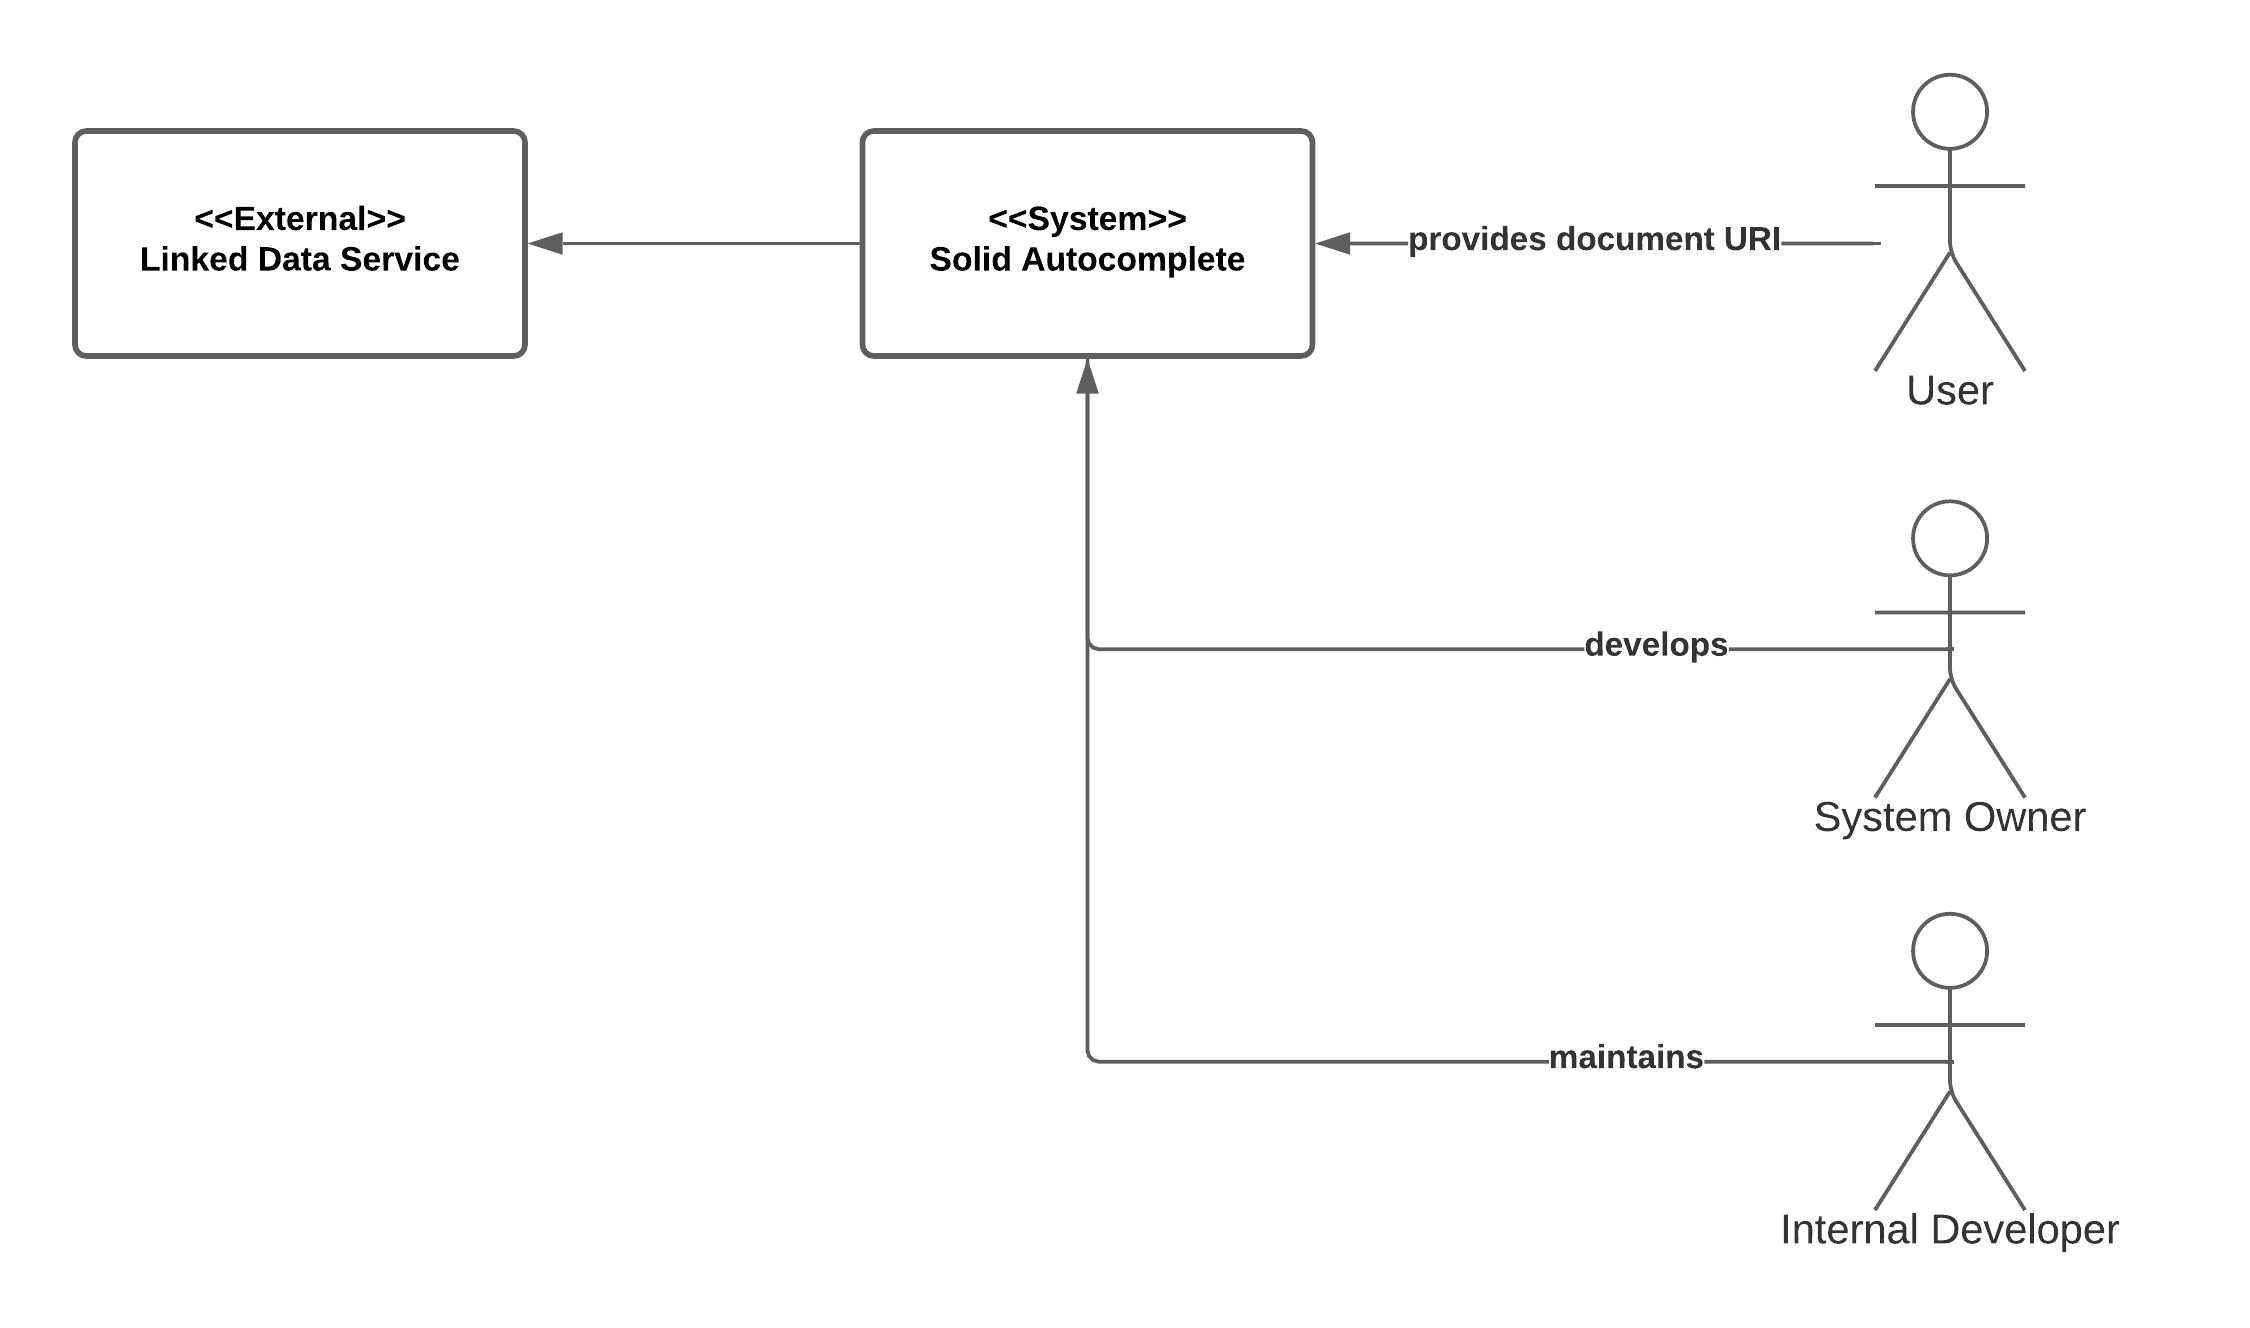
\includegraphics[width=0.8\textwidth]{prototype/graphs/poc-autocomplete-context_diagram.png}
    \caption{Context diagram showing users and external services of the system.}
    \label{fig:poc-autocomplete-context_diagram}
\end{figure}
\vspace{0.5cm}
\paragraph{Sequence Diagram}\mbox{}\\

The following succeeding diagram shows the sequential flow through the system upon initialization and button press. The focus was laid in the diagram to show the request/response cycles in the infrastructure. 

\begin{figure}[H]
    \centering
    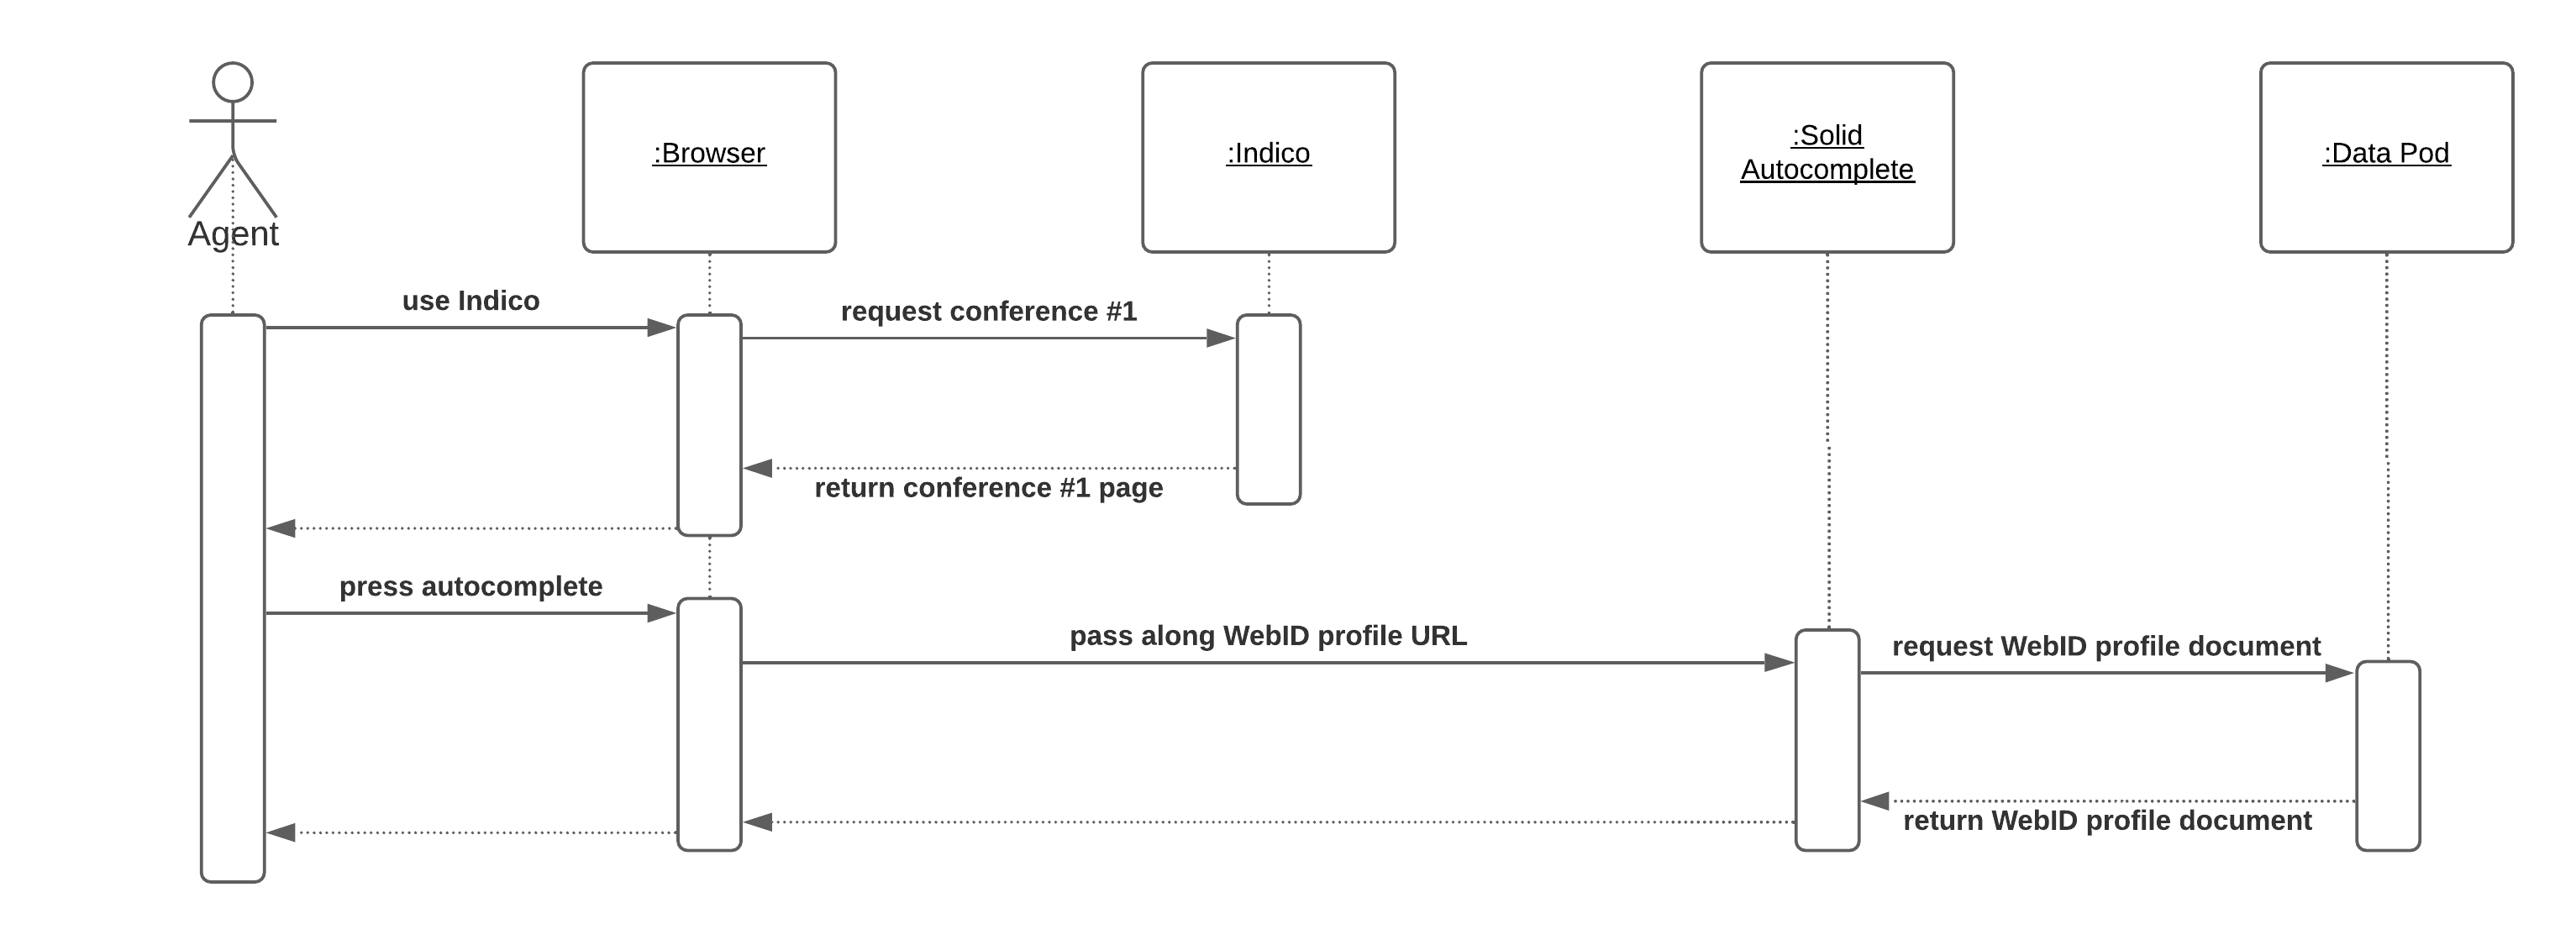
\includegraphics[width=\textwidth]{prototype/graphs/poc-conference_registration-autocomplete-sequence_diagram.png}
    \caption{Sequence diagram showing the sequential process through pulling in data from a data pod.}
    \label{fig:poc-conference_registration-autocomplete-sequence_diagram}
\end{figure}

\vspace{0.5cm}
\paragraph{Stakeholders}\mbox{}\\

Both modules were established with the same group of people and therefore carried the same set of stakeholders. The stakeholders defined in the section of the first \gls{poc} can be found here \ref{poc1-stakeholders}.
\vspace{0.5cm}
\paragraph{Drivers}\mbox{}\\

The drivers for this architecture endure the same as well. A system that operates on a form where sensitive data is exposed needs a high level of security -- under no circumstance should traffic be intercepted and leak any of such information. The performance for this module is also essential, as conferences tend to open their registration at a particular time, with high traffic spikes at those times of registration opening or announcements. The same reasoning as before applies to the \textit{Usability} of the module. Software design should be as simple as possible for the user to interact with, and ideally, a user should not even notice a difference from traditional practices.

\begin{enumerate}
    \item Security
    \item Performance
    \item Usability
\end{enumerate}

\subsubsection{User Interface}\mbox{}\\

The \gls{ui} for this module is moderately limited as it only requires an input field for the user to provide the \gls{uri} of where to find an \gls{rdf} document. The \gls{rdf} document fills in the registration form, an action button, and then a design for when two values on input are probable.

\begin{figure}[H]
    \centering
    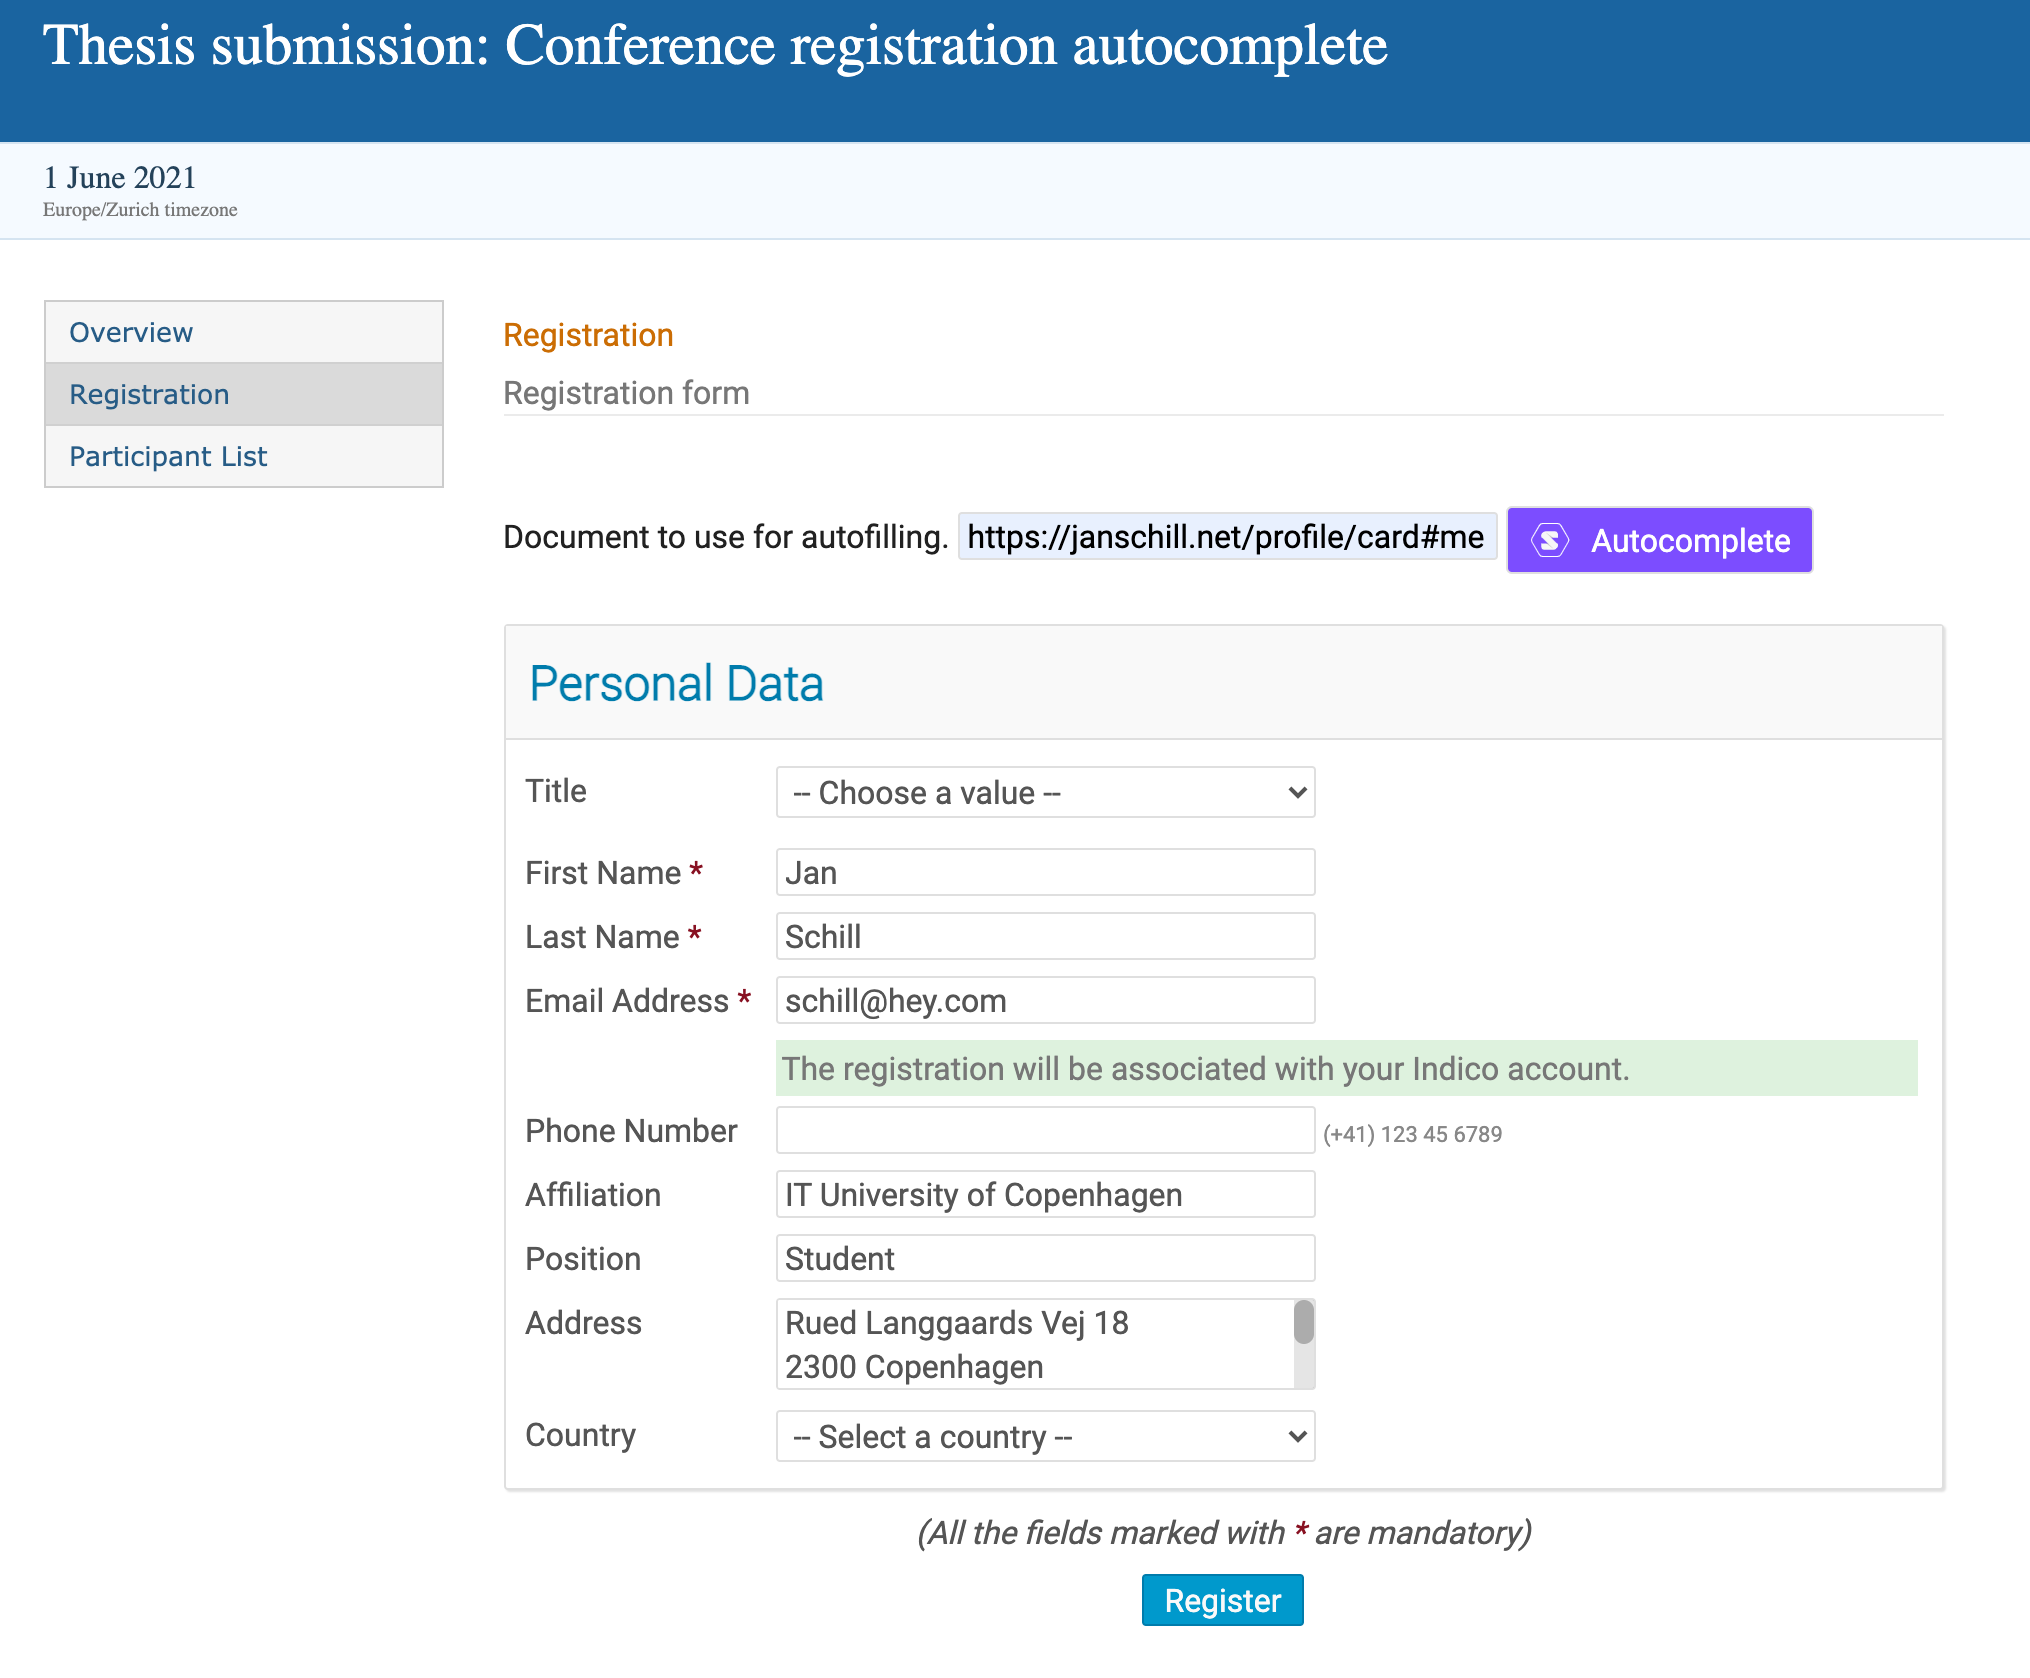
\includegraphics[width=0.75\textwidth]{prototype/poc-solid-autocomplete-conference-registration.png}
    \caption{\gls{ui} showing the autocomplete module.}
    \label{fig:poc-solid-autocomplete-conference-registration}
\end{figure}

\begin{figure}[H]
    \centering
    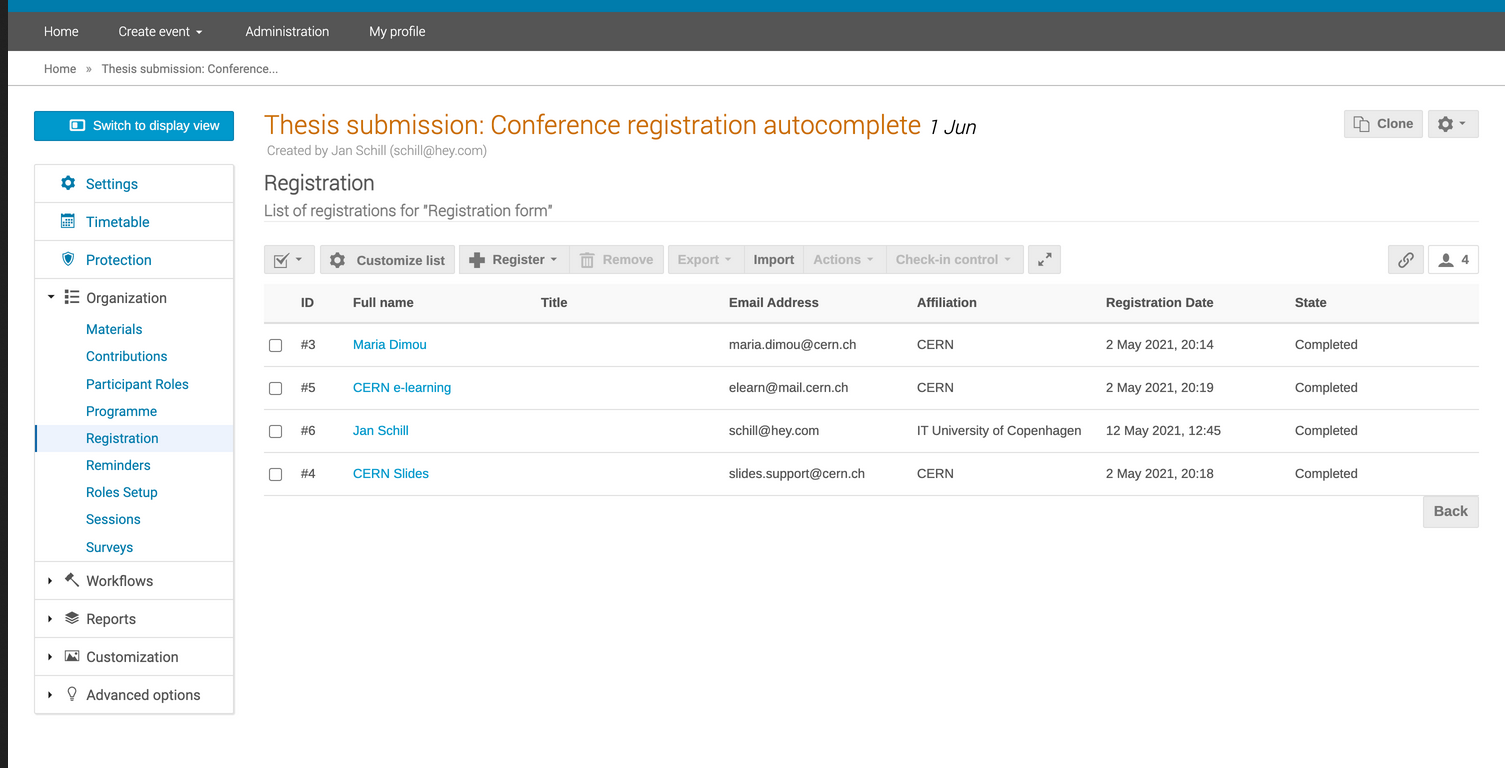
\includegraphics[width=0.75\textwidth]{prototype/poc-solid-autocomplete-conference-registration-attendees.png}
    \caption{The Indico control panel showing registered users.}
    \label{fig:poc-solid-autocomplete-conference-registration-attendees}
\end{figure}

\subsubsection{Design}\label{poc2:design}\mbox{}\\

The following section will shed light on the design decision made in sketching out the module's architecture and developing the system. It will introduce the different challenges and how they were overcome. Primarily, it will explain what led to the change of core functionality of the module. In the next section, the choices will be analyzed more explicitly.
\vspace{0.5cm}
\paragraph{Mapping Structured Data To \gls{html} Inputs}\mbox{}\\

A great benefit of using Linked Data is its semantic structure and the interoperability it brings when using in systems supporting it. Linked Data means the data uses shared vocabularies to be described and reasoned about by machines and can be moved from one system into another and seamlessly integrated. Indico does not use any standard \gls{rdf} features and can therefore not extract any of those benefits. Because of this, no straightforward way of mapping the incoming data from the data pod to the inputs exist, but a few options are feasible.

\begin{enumerate}
    \item Enrich the form with some descriptive indicator
    \item Parse and process existing values of attributes and labels
\end{enumerate}

In the \gls{html} specification, an \texttt{autocomplete} attribute exists, which browsers use to prefill data from previously used values \cite{html-spec}. The value of the \texttt{autocomplete} key-value pair describes the input and what data is to be expected.

\begin{lstlisting}[language=Other,columns=fullflexible, caption={Autocomplete attribute on input field}, label={lst:autocomplete-input}]
<form method=post action="/">
  <p><label>Full name: <input type=text autocomplete=name></label>
  <p><label>Credit card number: <input type=text inputmode=numeric autocomplete=cc-number></label>
  <p><label>Expiry Date: <input type=month autocomplete=cc-exp></label>
  <p><input type=submit value="Submit">
</form>
\end{lstlisting}

In listing \ref{lst:autocomplete-input}, the browser suggests cached values when the user clicks into an input. This functionality is the perfect indicator to \textit{autofill} form inputs. Unfortunately, this attribute is not being utilized in Indico. Another and even better approach would be to annotate the input fields straight up with the vocabulary of Schema.org \cite{schema-org}. The mapping of the input fields and the fetched Turtle resource could then happen directly using the \textit{predicates} of both structured formats. To change the AngularJS form and implement new features into Indico were already established not to be viable. Nevertheless, the \texttt{autocomplete} feature shall be kept in mind.

Without being able to extract from the \texttt{autocomplete} attribute within Indico, it shall still be implemented and used, as other systems might use the attribute. Other means of extracting some information from the form are the ID and name attributes or even the \texttt{TextNode} of the input label. The ID and name are often equipped with information about the input they are defined on. These values and the label node's value can be extracted and mapped against a dictionary of key-value pairs to determine what the input is supposed to be filled.

\begin{figure}[H]
    \centering
    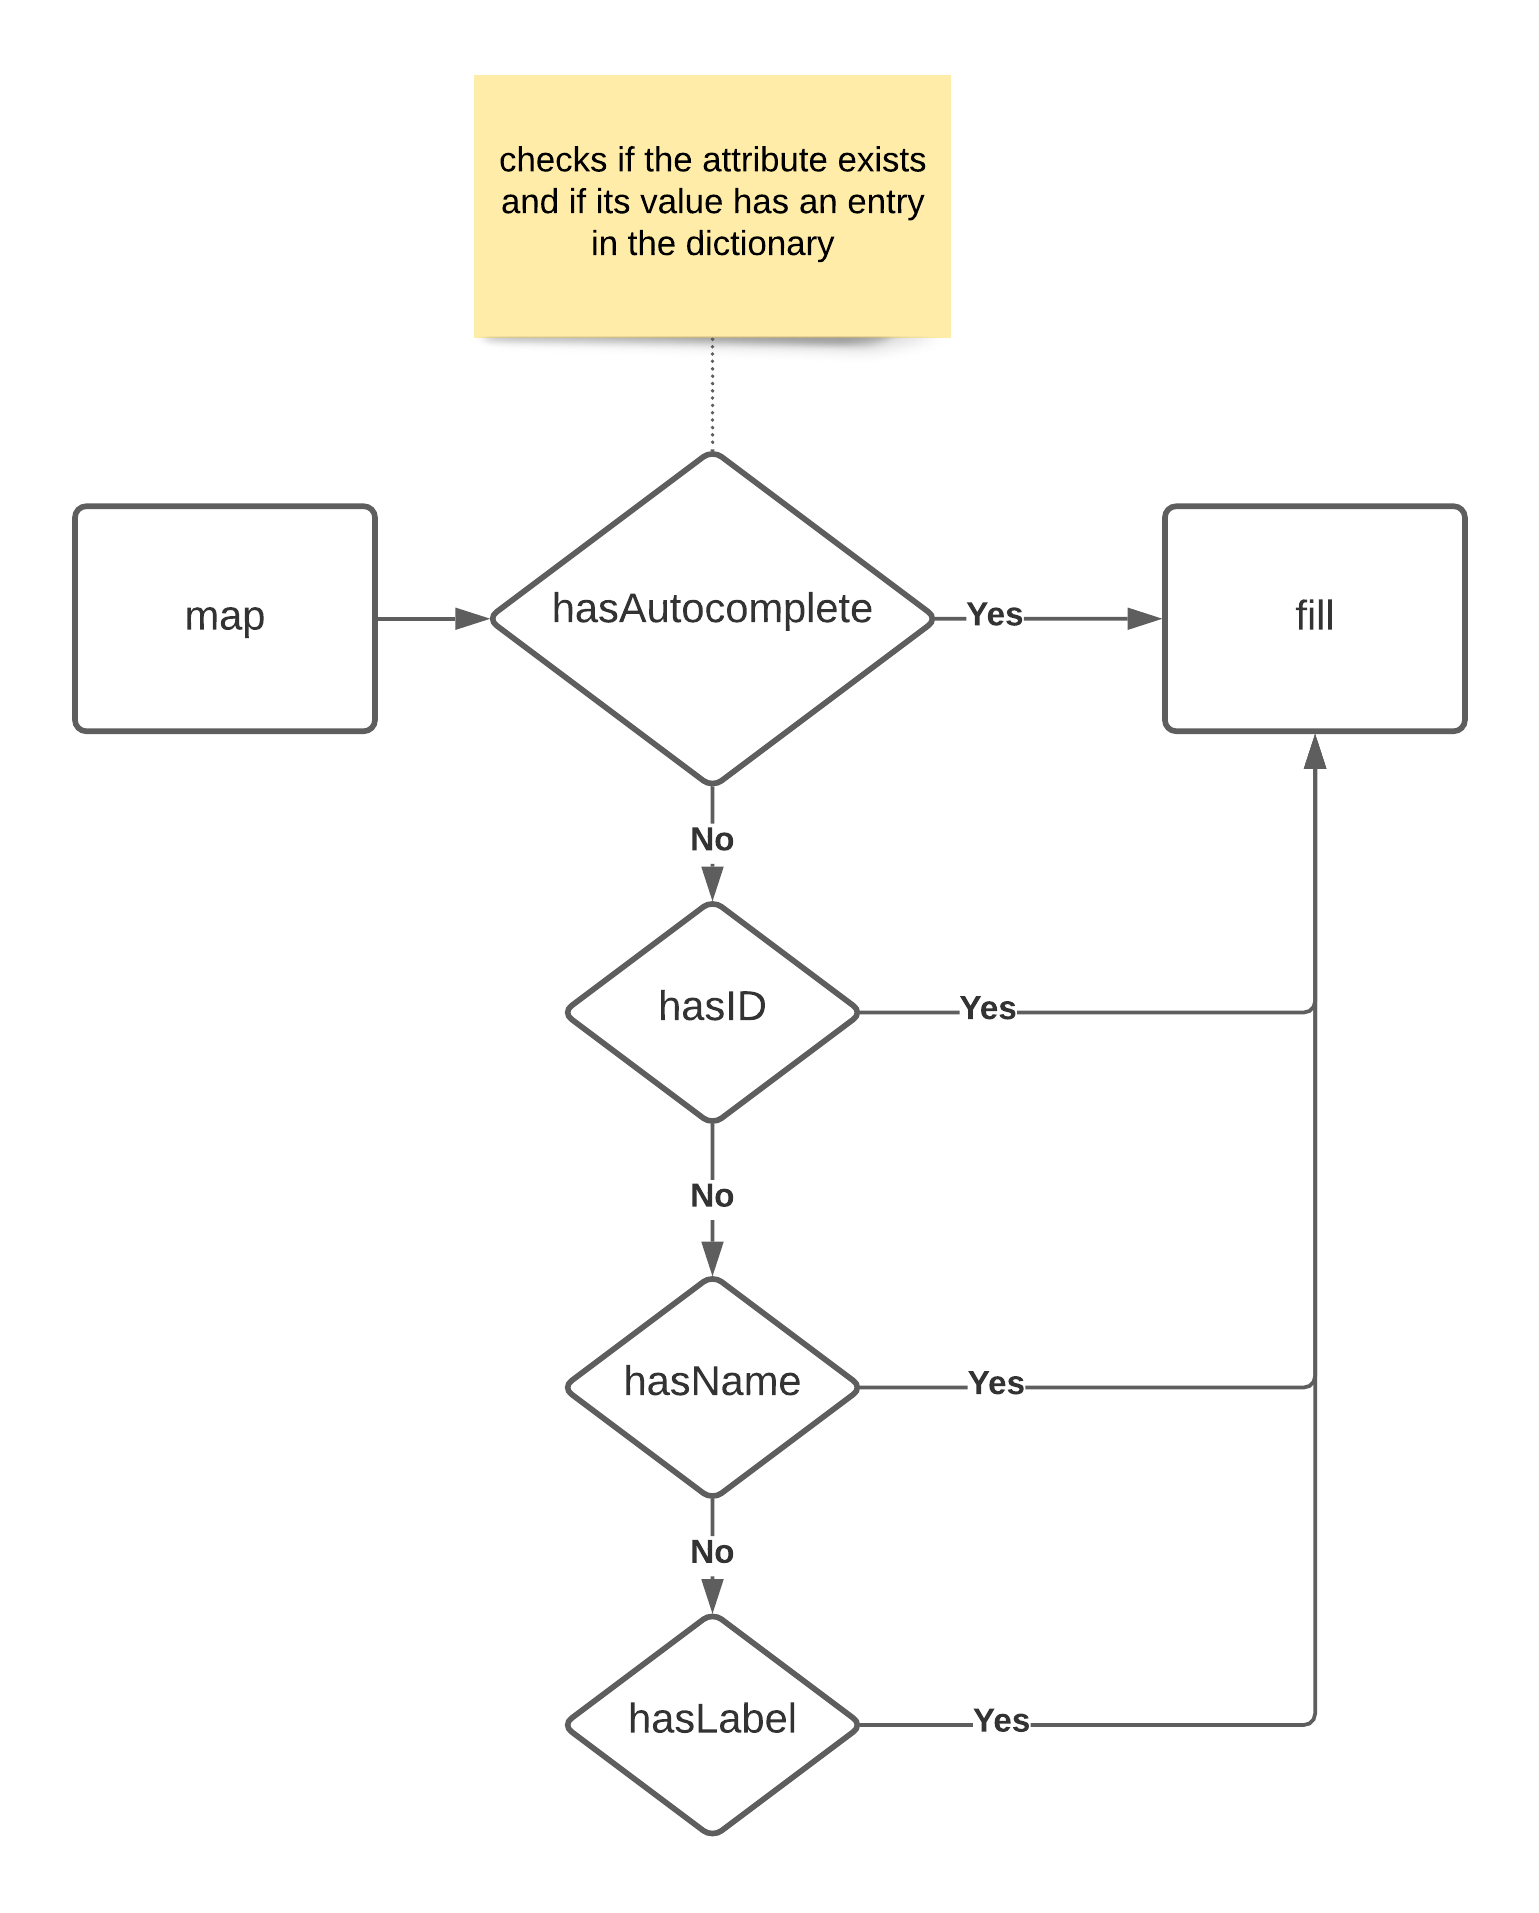
\includegraphics[width=0.5\textwidth]{prototype/graphs/poc-autocomplete-mapping-flow.png}
    \caption{The flow to find a source for dictionary mapping.}
    \label{fig:poc-autocomplete-mapping-flow}
\end{figure}

A possible mapping of address information could look like as in listing \ref{lst:autocomplete-mapping}. The implementation shows a \gls{js} implementation where the key in the \texttt{address} object is the possibly extracted values from the different techniques described above. The value is in this example the vCARD \cite{vcard-spec} equivalent. \gls{nss} uses vCARD to convey the information in the WebID profile document.

\begin{lstlisting}[language=Other,columns=fullflexible, caption={Dictionary to map extracted values with predicates from Turtle resource}, label={lst:autocomplete-mapping}]
const address = {
  address: 'full_address',
  country: VCARD.country_name.value,
  countryName: VCARD.country_name.value,
  region: VCARD.region.value,
  locality: VCARD.locality.value,
  city: VCARD.locality.value,
  streetAddress: VCARD.street_address.value,
  street: VCARD.street_address.value,
  postalCode: VCARD.postal_code.value
}
\end{lstlisting}

Listing \ref{lst:webid-address} shows part of the WebID profile document where the address of an agent is described.

\begin{lstlisting}[language=Other,columns=fullflexible, caption={Extraction from WebID profile document showing address.}, label={lst:webid-address}]
@prefix : <#>.
@prefix n: <http://www.w3.org/2006/vcard/ns#>.
# ...
:id1614172452178
  n:country-name "Denmark";
  n:locality "Copenhagen";
  n:postal-code "2300";
  n:region "Zealand";
  n:street-address "Rued Langgaards Vej 18". 
# ...
:me n:hasAddress :id1614172452178;
# ...
\end{lstlisting}

\vspace{0.5cm}
\subsubsection{Integration With Indico}\mbox{}\\

A few challenges arose when integrating the module with Indico. A critical issue is that the form is not being rendered on the server and then served as \gls{html} in the response body as expected. Another challenge was when programmatically filling in the input fields of the inputs; the frontend form validation would not detect a change in the input values and thus would think no input value is given.

\vspace{0.5cm}
\paragraph{Bind to Dynamically Created Form}\label{poc2-bind}\mbox{}\\

Indico builds the registration form dynamically using a frontend library called AngularJS \cite{angularjs}. A dynamically rendered form introduces the challenge of interacting with it using \gls{js}. Frontend libraries that either create new or modify existing \gls{dom} nodes need to wait until the complete \gls{dom} tree is loaded. They bind to one \gls{dom} node from the initially served \gls{html} document and then do their operations on this node. Meaning, AngularJS waits until the whole \gls{html} document is parsed and rendered in the browser and then starts creating its form from scratch, which is then being rendered by the browser. The problem with this is to operate on the form, which is necessary for the module to read the form inputs and labels and set their values. The \gls{js} code from this prototype needs to know when the browser rendered the form successfully. Three options are possible to achieve this.

\begin{enumerate}
    \item Implement the autocomplete functionality in the existing AngularJS form code
    \item Dispatch an event to notify the autocomplete module the form has been rendered
    \item Use the \texttt{MutationObserver} to detect the form creation
\end{enumerate}

Solutions 1 and 2 both involve the need to work with the AngularJS form, which is written in a legacy version and was recommended by an Indico developer to -- if possible -- be avoided. Indico developers also plan on removing AngularJS altogether and replace it with a more popular frontend framework. Therefore, option 3 was chosen even though a \texttt{MutationObserver} instance might add performance degradation to the page load \cite{dom-spec}. The performance shall not be analyzed more carefully as it is not relevant to prove the prototype's realization.

The \texttt{MutationObserver} is initialized as soon as the \gls{dom} is rendered; it then takes a node as a target to observe and registers all modifications on this node: the creation of children nodes in it, updates to the node itself, or any other modifications. In order to reduce computation on nodes that do not need to be observed, a suitable \gls{dom} element is needed. This node needs to exist when the \gls{dom} is loaded and needs to contain the final form node. The finally rendered \gls{html} form has an ID. The \texttt{MutationObserver} can use this ID to grab the target node and scope the observations.

\begin{lstlisting}[language=Other,columns=fullflexible, caption={Observe function in Indico}, label={lst:indico-observe}]
function observeFormCreation() {
  // ID of the AngularJS form, its creation needs to be observed
  const formId = 'registrationForm';
  // Candidate to limit observing scope
  const $conferencePage = document.querySelector('.conference-page');
  const targetNode = $conferencePage;
  // Only observe nodes, not attributes
  const config = {attributes: false, childList: true, subtree: true};

  const callback = (mutationsList, observer) => {
    // Contains all mutations in the targetNode
    for (const mutation of mutationsList) {
      // Node has beed added or removed
      if (mutation.type === 'childList') {
        // Look at all added nodes
        for (const node of mutation.addedNodes) {
          // Look for the AngularJS form
          if (node.id === formId) {
            // Once found, stop observing
            observer.disconnect();
            // Initialize the autocomplete library
            const solidAutocomplete = new SolidAutocomplete({form: node});
            solidAutocomplete.createAutocompleteDomControls(node);
          }
        }
      }
    }
  };
  // Start observing
  const observer = new MutationObserver(callback);
  observer.observe(targetNode, config)
}
\end{lstlisting}

\vspace{0.5cm}
\paragraph{Detect Input Change for Frontend Validation}\label{poc2-detect-input}\mbox{}\\

Indico deploys a frontend validation to make sure it receives proper values for the form's inputs. Basic validation checks for the presence of values in required inputs. This way, Indico can render a hint on the input fields with invalid values, for example, when no input was given. It turns out Indico has \texttt{\gls{dom} Event Listeners}, which detect if an input field is clicked in and if it is receiving inputs through a user typing in it. This validation implementation does not notice when changing the value of the \texttt{value} attribute of an input node, thus complaining when setting the values through \gls{js}.

\begin{lstlisting}[language=Other,columns=fullflexible, caption={Changing the value of an input node.}, label={lst:input-change}]
const formInputField = document.querySelector('.exampleFormInput')
formInputField.value = 'New value'
\end{lstlisting}

The example code in listing \ref{lst:input-change} would not be detected by Indico and would render a missing value hint upon submission.

Two ways of fixing the problem are conceivable.

\begin{enumerate}
    \item Change Indico frontend validation to detect value change
    \item Dispatch event when setting values in the autocomplete module
\end{enumerate}

Changing the Indico frontend validation might be more time-consuming than anticipated and is therefore not viable; it is also unknown if the Indico development team wants a change in the first place. The idea for a working implementation is to validate on submission of the form instead of validation when a change on the input is detected. The problem with the used \texttt{oninput} event is that it does not see when the value is set programmatically. If the validation is only happening when the values are tried to be sent to the server by submission, the input values can be parsed, and the correct value is detected -- no matter how it was set. 

The other and also picked solution is to trigger the \texttt{oninput} event listened to by the Indico validation. The event dispatch needs to happen as soon the values are set within the module, and because this occurs in the module and the module is a self-contained module without any knowledge of Indico, the module should not be directly changed but instead, allow a callback function to be passed to it and then execute when appropriate.

\begin{lstlisting}[language=Other,columns=fullflexible, caption={Dispatching the \texttt{oninput} event within a callback.}, label={lst:oninput-callback}]
function triggerInputEvent(inputs) {
  for (let i = 0; i < inputs.length; i++) {
    const element = inputs[i];
    [element, element.parentNode].forEach(node => {
      if ('createEvent' in document) {
        const evt = document.createEvent('HTMLEvents');
        evt.initEvent('input', false, true);
        node.dispatchEvent(evt);
      } else {
        node.fireEvent('oninput');
      }
    });
  }
}
\end{lstlisting}

\subsubsection{Evaluation}\mbox{}\\

Like with the first \gls{poc} from a section before \ref{poc1}, this \gls{poc} shall be evaluated using the same motivation and framework. The stakeholders and \glspl{qa} continue to be as is. An 
TODO:
\vspace{0.5cm}
\paragraph{Metrics}\mbox{}\\

The previously picked \glspl{qa} are as follows:

\begin{enumerate}
    \item Security
    \item Performance
    \item Usability
\end{enumerate}

The \glspl{qas} to make the \glspl{qa} measurable allowing the analysis of health in the system's architecture:

\begin{enumerate}
    \item As a user, I expect to see the information from my WebID profile document when using the module
    \item As a user, I expect to have the choice of two available values
    \item As a user, I expect to be incapable of pulling in protected resources without authenticating myself
\end{enumerate}
\vspace{0.5cm}
\paragraph{Levels}\mbox{}\\

The evaluation uses the same levels 1 to 5 as in the first evaluation \ref{section:poc1-evaluation} to rate the architecture of this system.
\vspace{0.5cm}
\paragraph{Components}\mbox{}\\

This module is compared to the other module, relatively small, and does not contain multiple packages. It forms through the three major classes \texttt{Picker}, \texttt{Mapper}, and \texttt{Filler}. These three classes find all relevant input fields from the application; secondly, maps the input fields with the available data fetched using the \texttt{DataFetcher} class; thirdly, it fills the available information through the mapping into the input fields.

\begin{figure}[H]
    \centering
    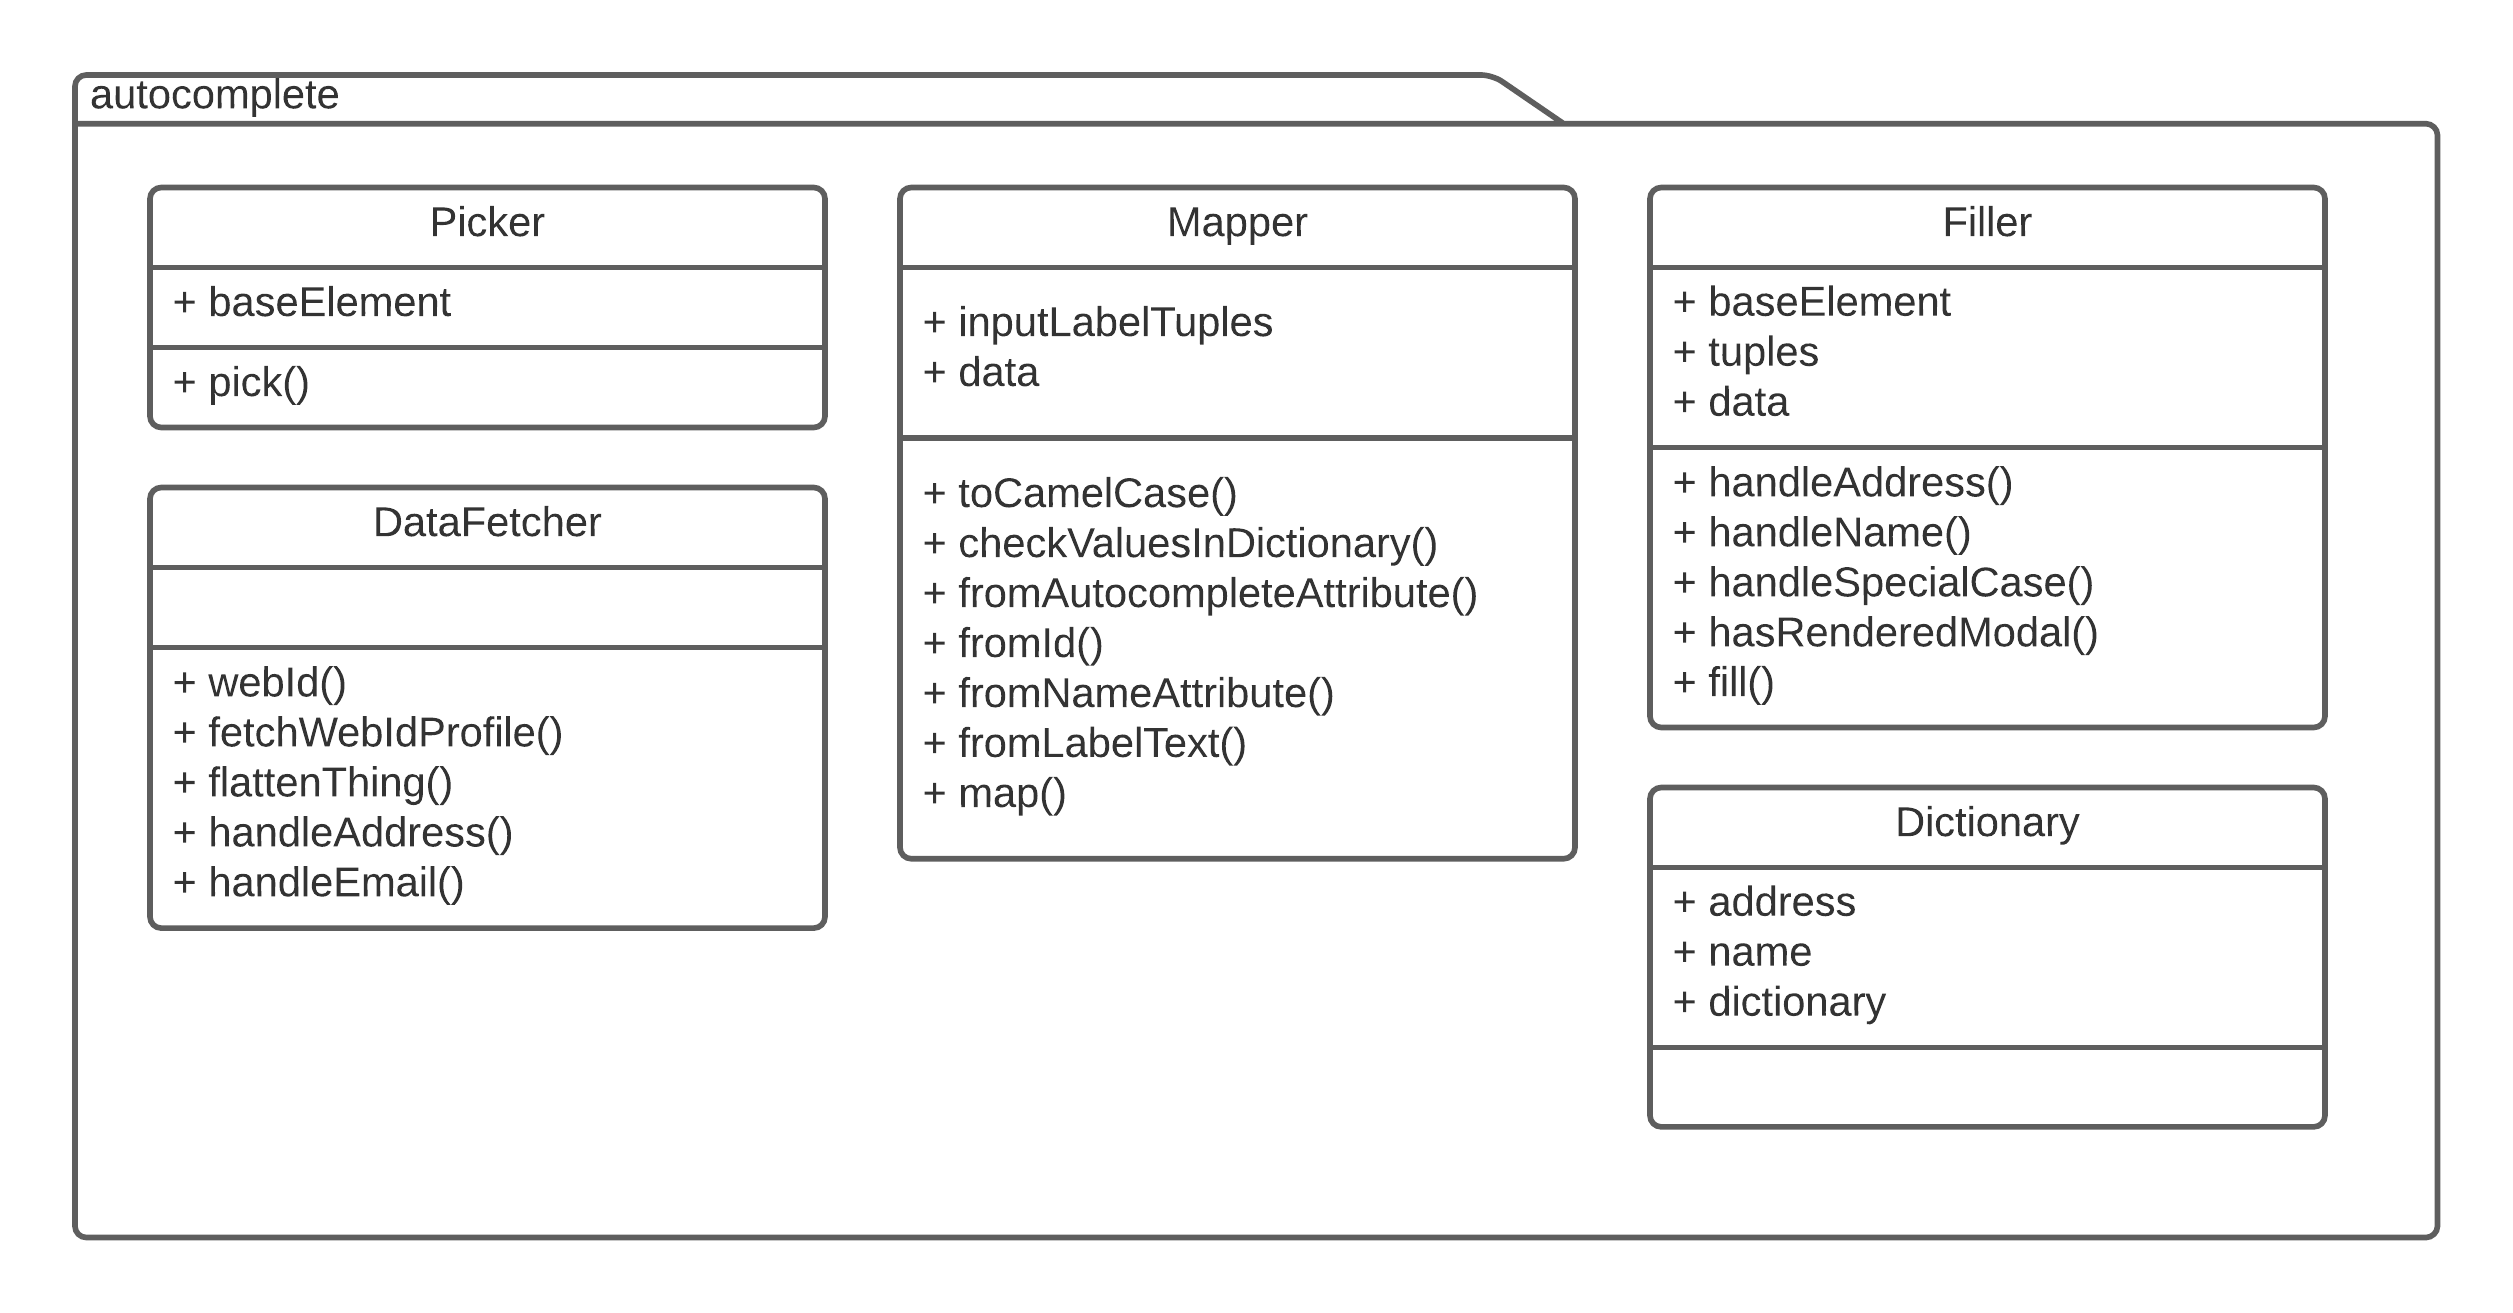
\includegraphics[width=0.7\textwidth]{prototype/graphs/poc-autocomplete-package.png}
    \caption{The classes in the autocomplete module.}
    \label{fig:poc-autocomplete-package}
\end{figure}
\vspace{0.5cm}
\paragraph{Evaluate}\mbox{}\\

\begin{itemize}
    \item \textbf{Target}: What is the desired quality level?
    \item \textbf{Current}: What is the current level?
    \item \textbf{Health}: Where are the most considerable quality problems?
    \item \textbf{Importance}: How important is it to move from current to target level?
    \item \textbf{Focus}: What are the most significant and most essential quality problems?
    \item \textbf{Valid level values}: 1, 2, 3, 4, 5 (higher equals better)
\end{itemize}

\textbf{Health} and \textbf{focus} are not set by the evaluator but instead calculated from other levels.

\begin{align*}
    \text{\textit{health}}&=5 - \text{\textit{max}}(0, (\text{\textit{target}} - \text{\textit{current}}))
\end{align*}
\vspace{-5mm}
\begin{align*}
    \text{\textit{focus}}&= \text{\textit{ceil}}((6 - \text{\textit{health}}) * \text{\textit{importance}}/5)
\end{align*}

\begin{enumerate}
    \item A user enters their WebID \gls{uri} and presses \textit{autocomplete}
    \item A user enters someone else's WebID \gls{uri} and presses \textit{autocomplete}
    \item A user enters a \gls{uri} with a protected resource and presses \textit{autocomplete}
    \item An adversary enters a \gls{uri} to a malicious document
\end{enumerate}

\begin{table}[h!]
    \centering
    \begin{tabular}{| l | c | c | c | c | c |} 
     \hline
     \texttt{autocomplete} & T & C & H & I & F \\
     \hline
     Security & 5 & 5 & 5 & 5 & \cellcolor{green!25}1\\
     \hline
     Performance & 3 & 3 & 5 & 3 & \cellcolor{green!25}2\\
     \hline
     Availability & 2 & 3 & 5 & 1 & \cellcolor{green!25}1\\
     \hline
     Usability & 5 & 2 & 2 & 5 & \cellcolor{red!25}4\\
     \hline
    \end{tabular}
    \vspace{0.75cm}
    \caption{Evaluation of the autocomplete module based on the \glspl{qas}}
    \label{table:poc2-evaluation}
\end{table}
\subsubsection{Analysis}\label{poc2:analysis}\mbox{}\\

The analysis of the second \gls{poc} will explain the evaluation matrix \ref{table:poc2-evaluation} and then focus on the original design idea and what led to a change of mind. It will do so by looking at the relevant modules in Indico that caused the direction for the \gls{poc} to alter.  The analysis will also look at what role Solid's design played in the abandonment of storing the registration data in data pods and effectively giving up usage control.

\vspace{0.5cm}

Because the module does not use any authentication libraries to allow users to log in or store any data in a data pod, it simply fetches public documents. The user interacting with the module decides what to fetch; no risk is involved. Regarding pulling in malicious documents from a trustworthy thought source, the module is embedded into Indico, which has validations and makes sure no malicious code is injected into their system.
The performance of the module is also in good shape. Only one request happens when the system is doing its tasks. The dictionary for the mapping of values uses the \gls{js} \texttt{Object} data type. It allows constant $\bigO(1)$ look-ups of values. See listing \ref{lst:autocomplete-mapping} to see an example data store of values. One area of improvement for the performance is the \texttt{MutationObserver} that was explained in paragraph \ref{poc2-bind}. Indico throws an event when all dynamically created \gls{dom} elements have been rendered, perfect for the module's binding to the Indico form. It was only later noticed that this event exists.
\vspace{0.5cm}
\paragraph{Iterations}\mbox{}\\

As mentioned before, this module went through two iterations of the design. Until creating the architecture of the actual module, it was undiscovered that the development of a module that sits on the registration form and allows decentralized storage is not viable. Figure \ref{fig:poc-conference_registration_flow-sideways} shows the same flow through the conference registration with Solid. It checks if the user wants to register regularly and let Indico have and handle the registration data or if the user wants to use their WebID and thus store the data in their data pod for maximum usage control.

\begin{figure}[H]
    \centering
    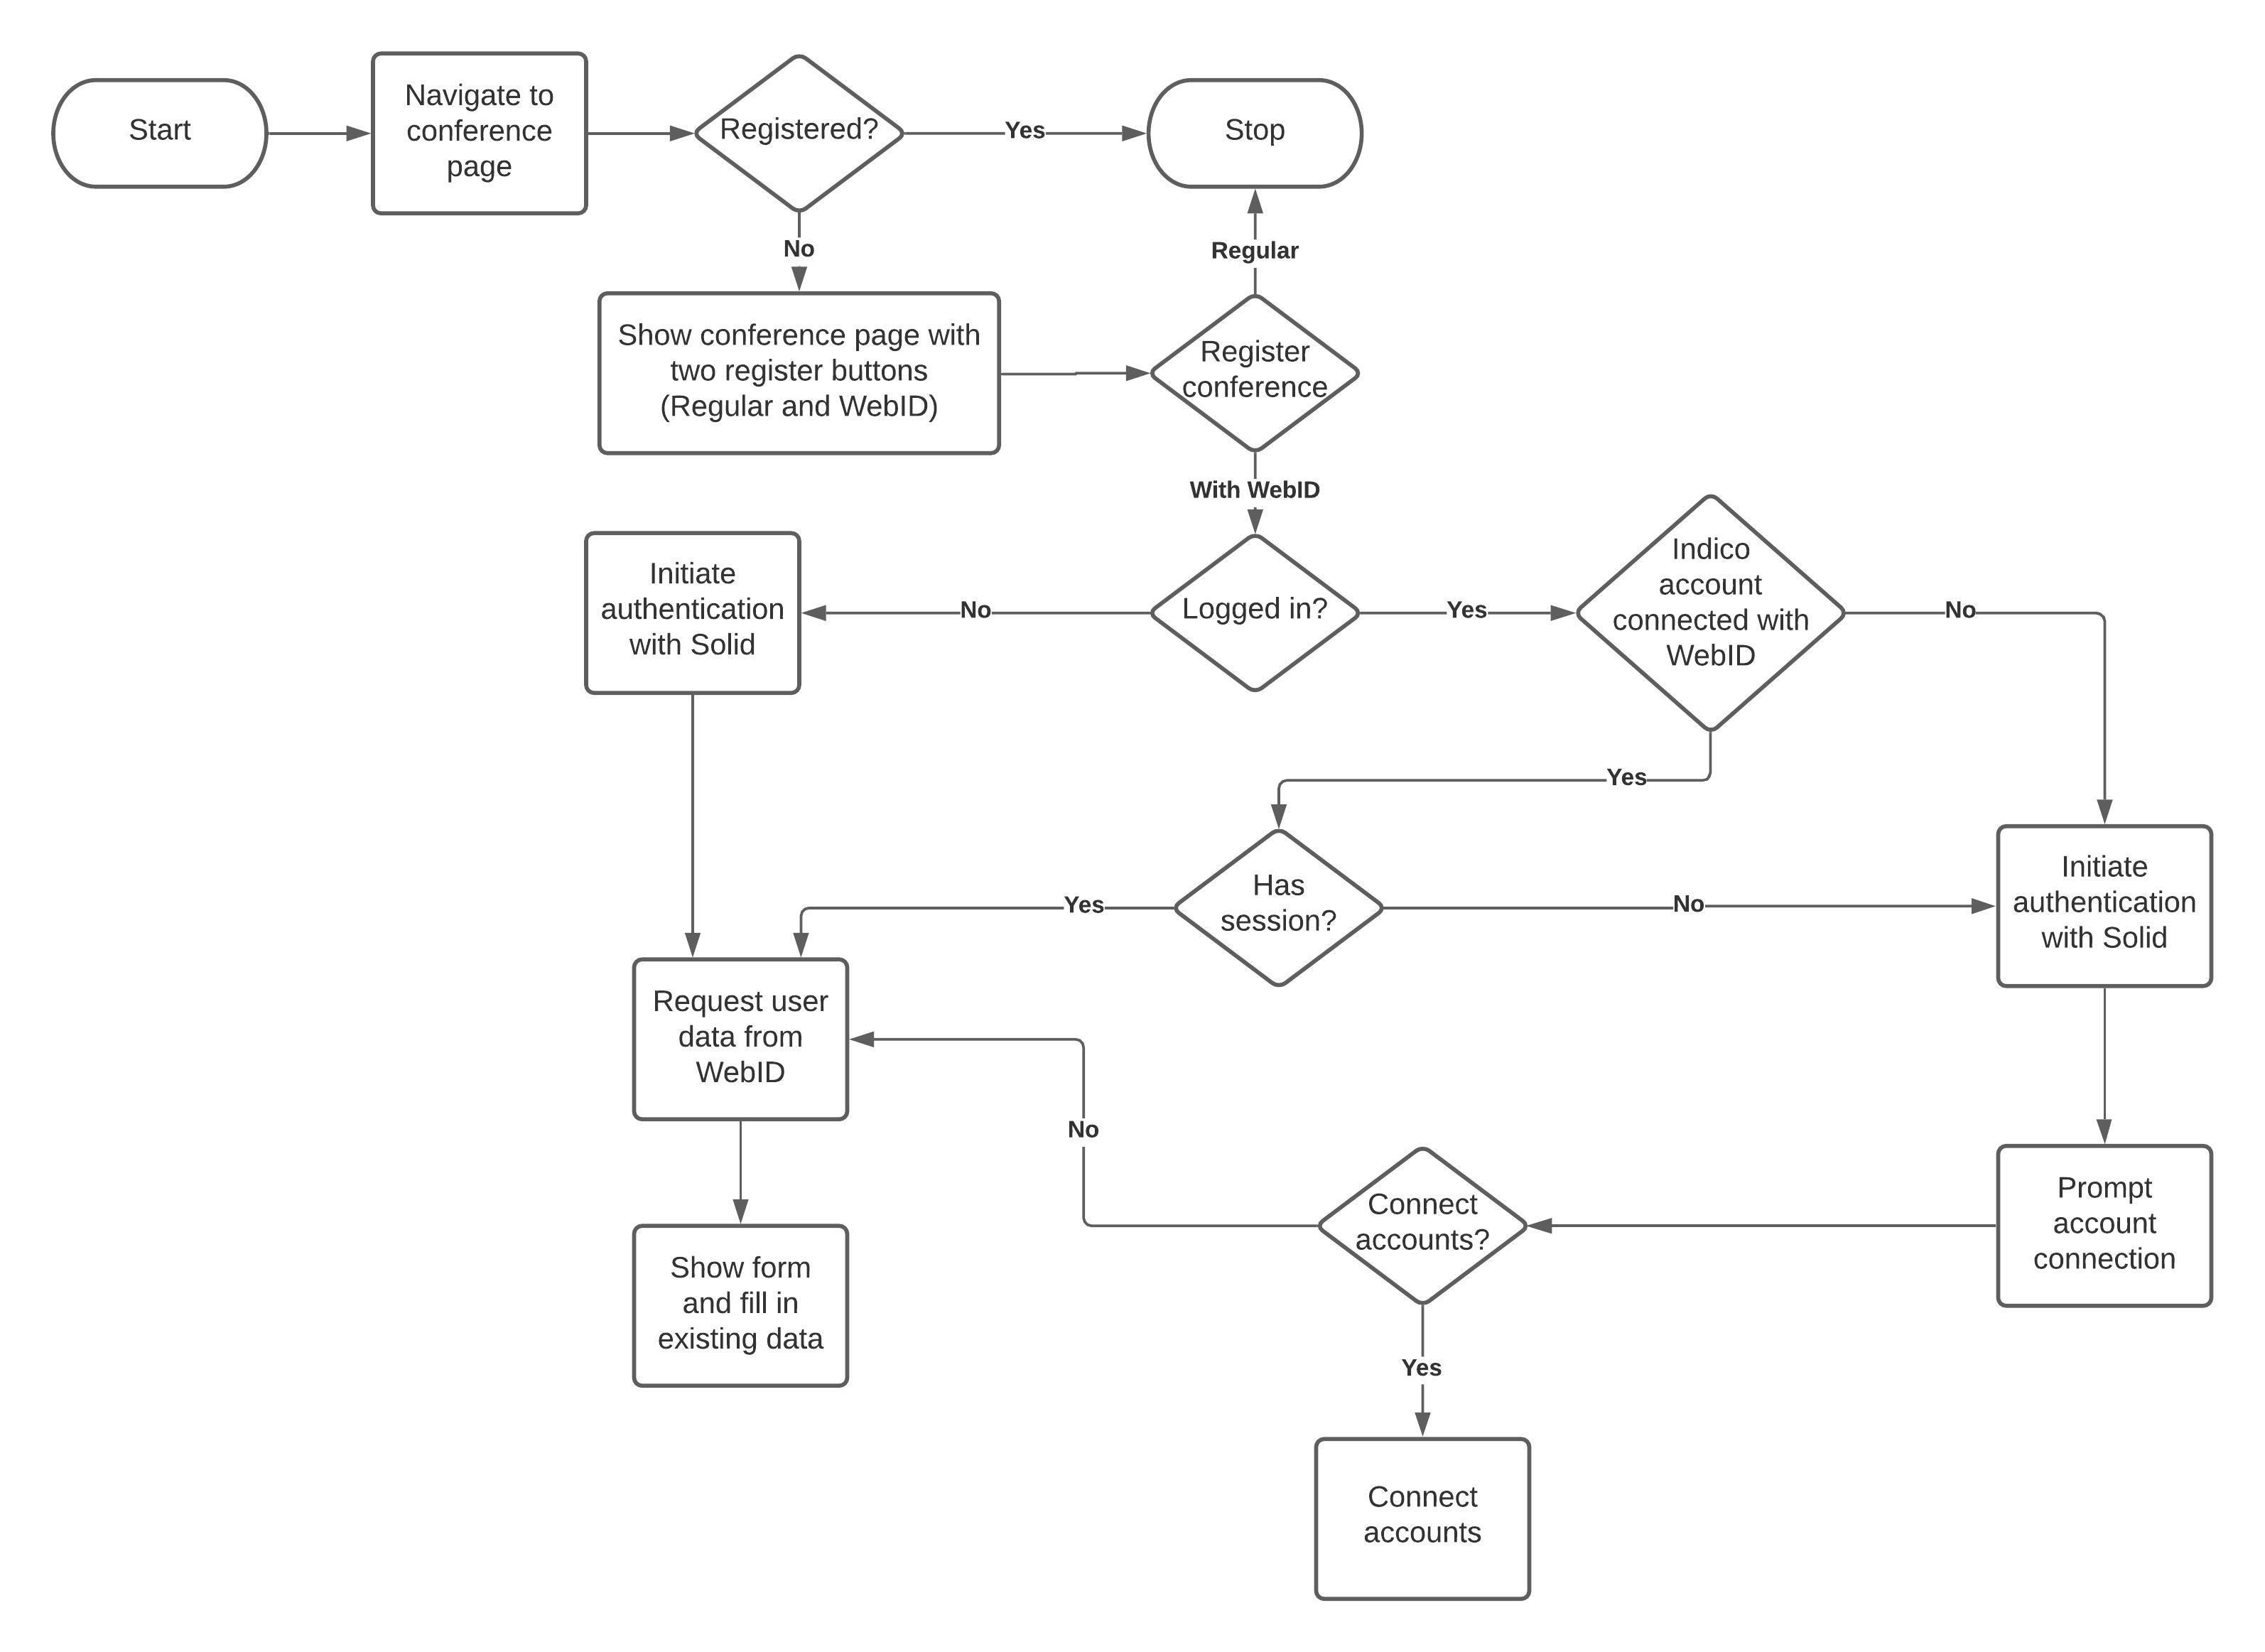
\includegraphics[width=1\textwidth]{prototype/graphs/poc-conference_registration_flow-sideways.jpeg}
    \caption{Flow through the registration flow using Solid account.}
    \label{fig:poc-conference_registration_flow-sideways}
\end{figure}

A few challenges were unidentified at this point but will be named and explained now.
\vspace{0.5cm}
\paragraph{Modification of Resource From Data Pod}\mbox{}\\

As also realized in the first \gls{poc}, when the application is decoupled from the data and receives it upon request, the application hands over the control. This shift of power is a core concept in Solid but problematic for Indico. The use-case of registration data differs with the handling of comments. Comments are often desired to be changed, and primarily comments are just presented in the \gls{ui}, and no other interaction or processing happens. Registration data is much more complex and requires a lot of processing, such as submitting abstracts. \textit{Call for abstracts} is a workflow in Indico, where conference speakers need to upload an abstract about the conference talk. Another is the requirement for processing in the field of payments in the registration. A registration form can offer users an option to book accommodation, for example. These fields are called \textit{billable} fields and are hooked into a checkout process. In Indico's management view of a conference, an administrator can check the status of these actions.

\begin{enumerate}
    \item What happens now if this data is not kept in Indico anymore?
    \item How is Indico validating that a registrant has paid their bookings if all registration information is kept outside of Indico?
    \item What happens to generated registration tickets or receipts when a user changes the name on their data pod?
\end{enumerate}

Indico allows the editing of the registration up until a set modification deadline; after it, the registration is frozen, and registrants cannot update input fields. It is necessary to have time to process the registrations, such as the booking of accommodation. The classic setup where every user has their data pod to store all this registration data would not work without additional functionality. A few things are imaginable.

\begin{itemize}
    \item Store a copy of the registration data in Indico and freeze the copy on the modification deadline.
    \item Only allow decentralized storage on data where a modification would not matter
\end{itemize}

Storing a copy of the data is an interesting idea. The freezing of the data would require Indico to also save the data in their data stores. If information is modified directly on the data pod, Indico is not necessarily notified by the change. If the user who changed the data on their data pod wants Indico to use the latest version for their copy, Indico would have to be either notified so it can fetch the new resource from the data pod; the change needs to happen through Indico’s web interface, so Indico can send the request to update it in the data pod, but also in their storage; Indico sends a request to all data pods on modification deadline day and updates the stored version. The latter solution needs validation so that existing is not replaced with corrupt or invalid data, and it is also questionable what happens when the data pod is unavailable. Still, the data shows a resignation from the conference or anything similar. How is it ensured that Indico and the user's intentions are aligned? The two systems need to be interconnected, and it needs to be clear when updates happen---availability and flow of communication or critical aspects for this success.
\vspace{0.5cm}
\paragraph{Communication Flow}\mbox{}\\

Not to cut off the previous issue, but to continue and nurture the flow aspect in Solid. One crucial feature of conferences and registration is reaching out to people to let them know about next year's conference. A user would ideally only consent to the conference where they had actively signed up. Hence, next year's conference would not be able to read the participant's list and connect with them, and even if the list would be visible, how does the new conference know how to ask for consent to reach out to them or do akin actions. Solid offers an \textit{inbox} and \textit{notifications} \cite{solid-inbox}, which allow anyone in the Solid ecosystem to connect and send a \textit{message} to a WebID. The reached-out agent gets a notification as soon as a new item is appended into their inbox. This pro-active initiation is not ideal, as the initiator does not know what data they can ask. Only when the owner actively says: “You are allowed to read this resource A and modify my resource B.” does the application know about the existence of the data.

Solid-Inbox seems to be a decent solution for the use-case of Indico reaching out to previous participants. Another suggestion would be to escalate the access scope for Indico and conferences and the agent. Meaning, when a user signs up for a conference, the registration asks for consent to allow future contacting.
TODO: more here
\vspace{0.5cm}
\paragraph{Performance of Large Conference}\mbox{}\\

The identical performance issue from the first \gls{poc} \ref{poc1} would arise in the management part of the conference. Storing the source of truth for hundreds of registrations without a local copy in a remote data pod would mean they would have to be fetched. Even with caching improvements, this would still be problematic and would not be feasible -- pods can be down or stored on slow web servers. To make this usable in Indico, a proxy is compulsory. The proxy would temporarily store the information and make it available in a single request for multiple conference managers on separate machines. Warming up the cache by requesting resources from hundreds of data pods would still take a long time. The key takeaway here is that Indico is also serving data to users. Indico is not only taking in the registration data and then processes it and enables some feature for a single user who is only interacting with his data. On the contrary, Indico also serves a subset of users, the conference managers, data. The progress of serving the data from others is the critical facet.
\vspace{0.5cm}
\paragraph{Payment on Input Fields}\mbox{}\\

TODO:


* Gave up usage control
  * Why it didn't work, and **what is necessary to make it work**
    * usage control
    * question the choice of Indico usage control
    * versioning of tag of personal data
* high-level constraints
* implementation
  * indico limits this
* if indico in this way or more generally

TODO:
1st iteration, save data in pod
2nd iteration, only pull data from pod

\vspace{0.5cm}
\paragraph{Availability of Crucial User Data}\mbox{}\\
